% \documentclass[fleqn,usenatbib]{mnras}
\documentclass[a4paper,11pt]{article}
\pdfoutput=1
\usepackage{jcappub}
\usepackage{newtxtext,newtxmath}
\usepackage[T1]{fontenc}
\usepackage{graphicx}
\usepackage{amsmath}
\usepackage{hyperref}
% \usepackage{amssymb}
% Allow "Thomas van Noord" and alike to be sorted by "N" etc. in the bibliography.
% Write the name in the bibliography as "\VAN{Noord}{Van}{van} Noord, Thomas"
\DeclareRobustCommand{\VAN}[3]{#2}
\let\VANthebibliography\thebibliography
\def\thebibliography{\DeclareRobustCommand{\VAN}[3]{##3}\VANthebibliography}

% martin comment function
\newcommand{\maf}[1]{{\textcolor{red}{[{\bf MAF}: #1]}}}
% mingfeng comment function
\newcommand{\mfh}[1]{{\textcolor{green}{[{\bf MFH}: #1]}}}
% simeon comment function
\newcommand{\spb}[1]{{\textcolor{magenta}{[{\bf SPB}: #1]}}}

% ming-feng emulator commands
\newcommand{\mfemu}{\texttt{MFEmulator}}     % i made the acronym, but not used a lot
\newcommand{\Data}{\mathcal{D}}
\newcommand{\gp}{\textsc{gp}}
\newcommand{\normal}{\mathcal{N}}
\newcommand{\GP}{\mathcal{GP}}
\newcommand{\thetavec}{\boldsymbol{\theta}}  % input parameters
\newcommand{\zvec}{\boldsymbol{z}}
\newcommand{\outputFunction}{Z}
\newcommand{\outputVector}{\zvec}            % output response
\newcommand{\outputVectorModel}{\zvec_\mathrm{model}}
\newcommand{\outputVectorObs}{\zvec_\mathrm{obs}}
\newcommand{\muvec}{\boldsymbol{\mu}}        % GP mean vector
\newcommand{\Kvec}{\boldsymbol{\mathrm{K}}}  % covariance matrix
\newcommand{\kvec}{\boldsymbol{k}}           % covariance vector
\newcommand{\Lya}{Lyman-$\alpha$ Forest}
\newcommand{\astrid}{\texttt{ASTRID}}

\newcommand{\apjs}{ApJ Supplement}
\newcommand{\apj}{ApJ}
\newcommand{\aap}{AAP}
\newcommand{\mnras}{MNRAS}
\newcommand{\prd}{PRD}
\newcommand{\gadget}{{\small GADGET}}
\newcommand{\mpgadget}{{\small MP-GADGET}}

\newcommand{\km}{k_{max}}

\newcommand{\vect}[1]
  {\mbox{\boldmath ${#1}$}}
\newcommand{\matr}[1]
  {\mbox{\bf \sf{#1}}}
\newcommand{\eq}[1]
  {Eq.~(\ref{equation:#1})}
\newcommand{\eqs}[1]
  {Eqs~(\ref{equation:#1})}
\newcommand{\sect}[1]
  {section~\ref{section:#1}}
\newcommand{\sects}[1]
  {sections~\ref{section:#1}}
\newcommand{\tabl}[1]
  {{\mbox Table~\ref{table:#1}}}
\newcommand{\tabls}[1]
  {{\mbox Tables~\ref{table:#1}}}
\newcommand{\fig}[1]
  {Fig.~\ref{Figure:#1}}
\newcommand{\figs}[1]
  {Figs.~\ref{Figure:#1}}
\newcommand{\sourcesection}[1]{\noindent {\em{#1}} ---}

\def\jcap{JCAP}        % Journal of Cosmology and Astro-Particle Physics

\newcommand{\Msun}{\, h^{-1} M_\odot}
\newcommand{\Zsun}{Z_\odot}
\newcommand{\NHunit}{cm$^{-2}$}
\newcommand{\sLLS}{\sigma_\mathrm{LLS}}
\newcommand{\Mpc}{\,\mathrm{Mpc}}
\newcommand{\Mpch}{\, h^{-1} \mathrm{Mpc}}
\newcommand{\kpch}{\, h^{-1}\mathrm{kpc}}
\newcommand{\hMpc}{\, h \mathrm{Mpc}^{-1}}
\newcommand{\kms}{km~s$^{-1}$}
\newcommand{\NHI}{N_\mathrm{HI}}

\newcommand{\edit}[1]{#1}

%opening
\title{A New Suite of Lyman-$\alpha$ Forest Simulations for Cosmology}

\author[a,1]{Martin Fernandez,\note{Corresponding author}}
\author[a]{Simeon Bird,}
\affiliation[a]{Department of Physics \& Astronomy, University of California, Riverside,\\900 University Avenue, Riverside, CA 92521, USA}

\emailAdd{mfern027@ucr.edu}
\emailAdd{sbird@ucr.edu}

\abstract{
We present a new suite of $42$ simulations of the Lyman-$\alpha$ forest, spanning an $8$-dimensional parameter space with $3$ cosmological parameters and $5$ astrophysical/thermal parameters. These simulations advance on earlier simulations suites by larger particle loads, by incorporating new physical models for hydrogen and helium reionization, and by self-consistently incorporating a model for AGN feedback. Parameters are chosen based on a Latin hypercube design and a Gaussian process is used to interpolate to arbitrary parameter combinations. Our simulation suite will be used to interpret existing Lyman-$\alpha$ forest 1D flux power spectra from SDSS and future DESI data releases.
}

\begin{document}

\maketitle

\section{Introduction}

Introduce the problem. Cite the previous simulation suites for the Lyman alpha forest. The purpose of a simulation suite is to compare to observational measurements. The main output of our suite is a set of medium resolution artificial flux power spectra, from which the flux power spectrum may be generated. In this paper we describe the simulation suite we have run and defer description of the likelihood function to upcoming work.

\section{Simulation Parameters}

We use a suite of full physics simulations with star formation, stellar winds and AGN feedback. Our simulations are based on the model used in the \astrid~simulation described in \cite{Bird:2022}. In this Section we describe the various models, focussing on places where we have modified the model from that described in \cite{Bird:2022}. We discuss the models of hydrogen reionization, helium reionization, AGN feedback and star formation.

We use full physics simulations primarily because it allows us to incorporate our AGN feedback model self-consistently into the code, rather than with a post-processing correction. This allows us to ensure that potential parameter degeneracies between AGN feedback and cosmological parameters are included. Ref~\cite{find} has shown that the main degeneracy for the matter power spectrum is between AGN feedback and the fraction of matter in baryons, $\Omega_b / \Omega_0$. However, our main observable is the \Lya~forest which is sensitive to the thermal state of the gas and thus the heating effect of the AGN feedback rather than its ability to remove gas from the halo. It also allows us to self-consistently include the effect of self-shielded gas in the modelling, by producing DLAs in our spectral code and removing them, as in the observational analysis. We stress that these are likely small effects and we certainly do not wish to imply that quick \Lya~models are inadequate for current data. However, with current simulation codes the speed difference between the quick \Lya~and full physics simulations is not as significant as in earlier simulations, and is less than a factor of $2$ (dependent somewhat on cosmological parameters). Furthermore, using full physics simulations allows our suite to be used for other applications in future.

We also include models for hydrogen and helium reionization.

\subsection{Gravity and Hydrodynamics}

\subsection{Helium and Hydrogen Reionization}

Mean temperature plot for the helium reionization model parameters.

\begin{figure*}
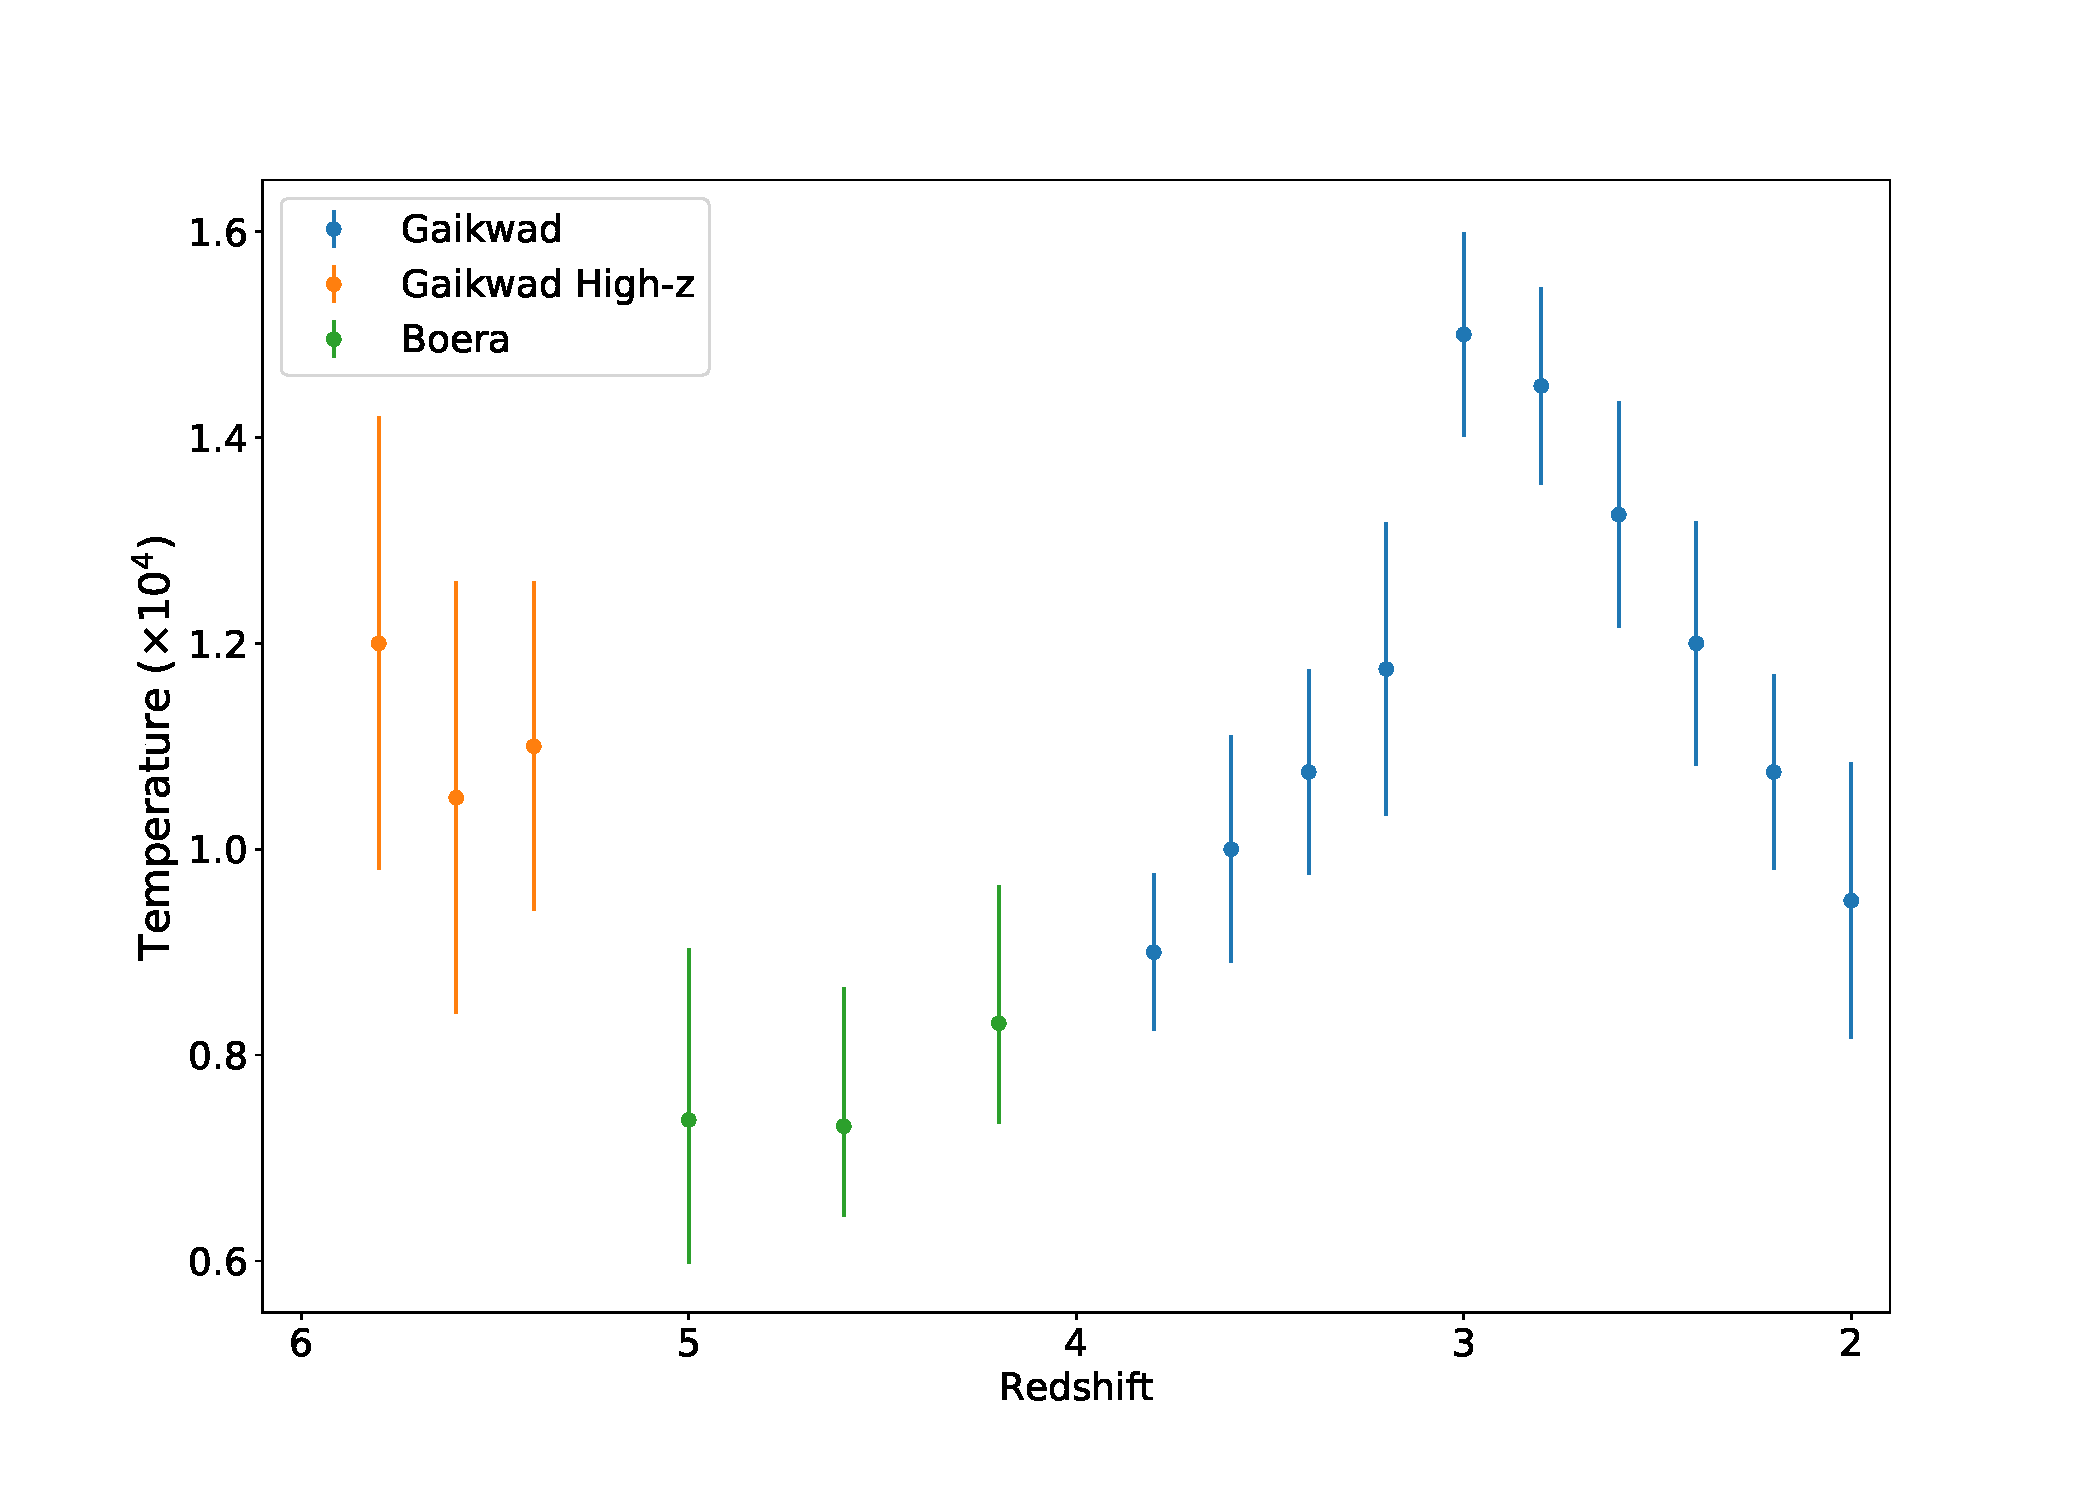
\includegraphics[width=0.45\textwidth]{figures/temp_observed.pdf}
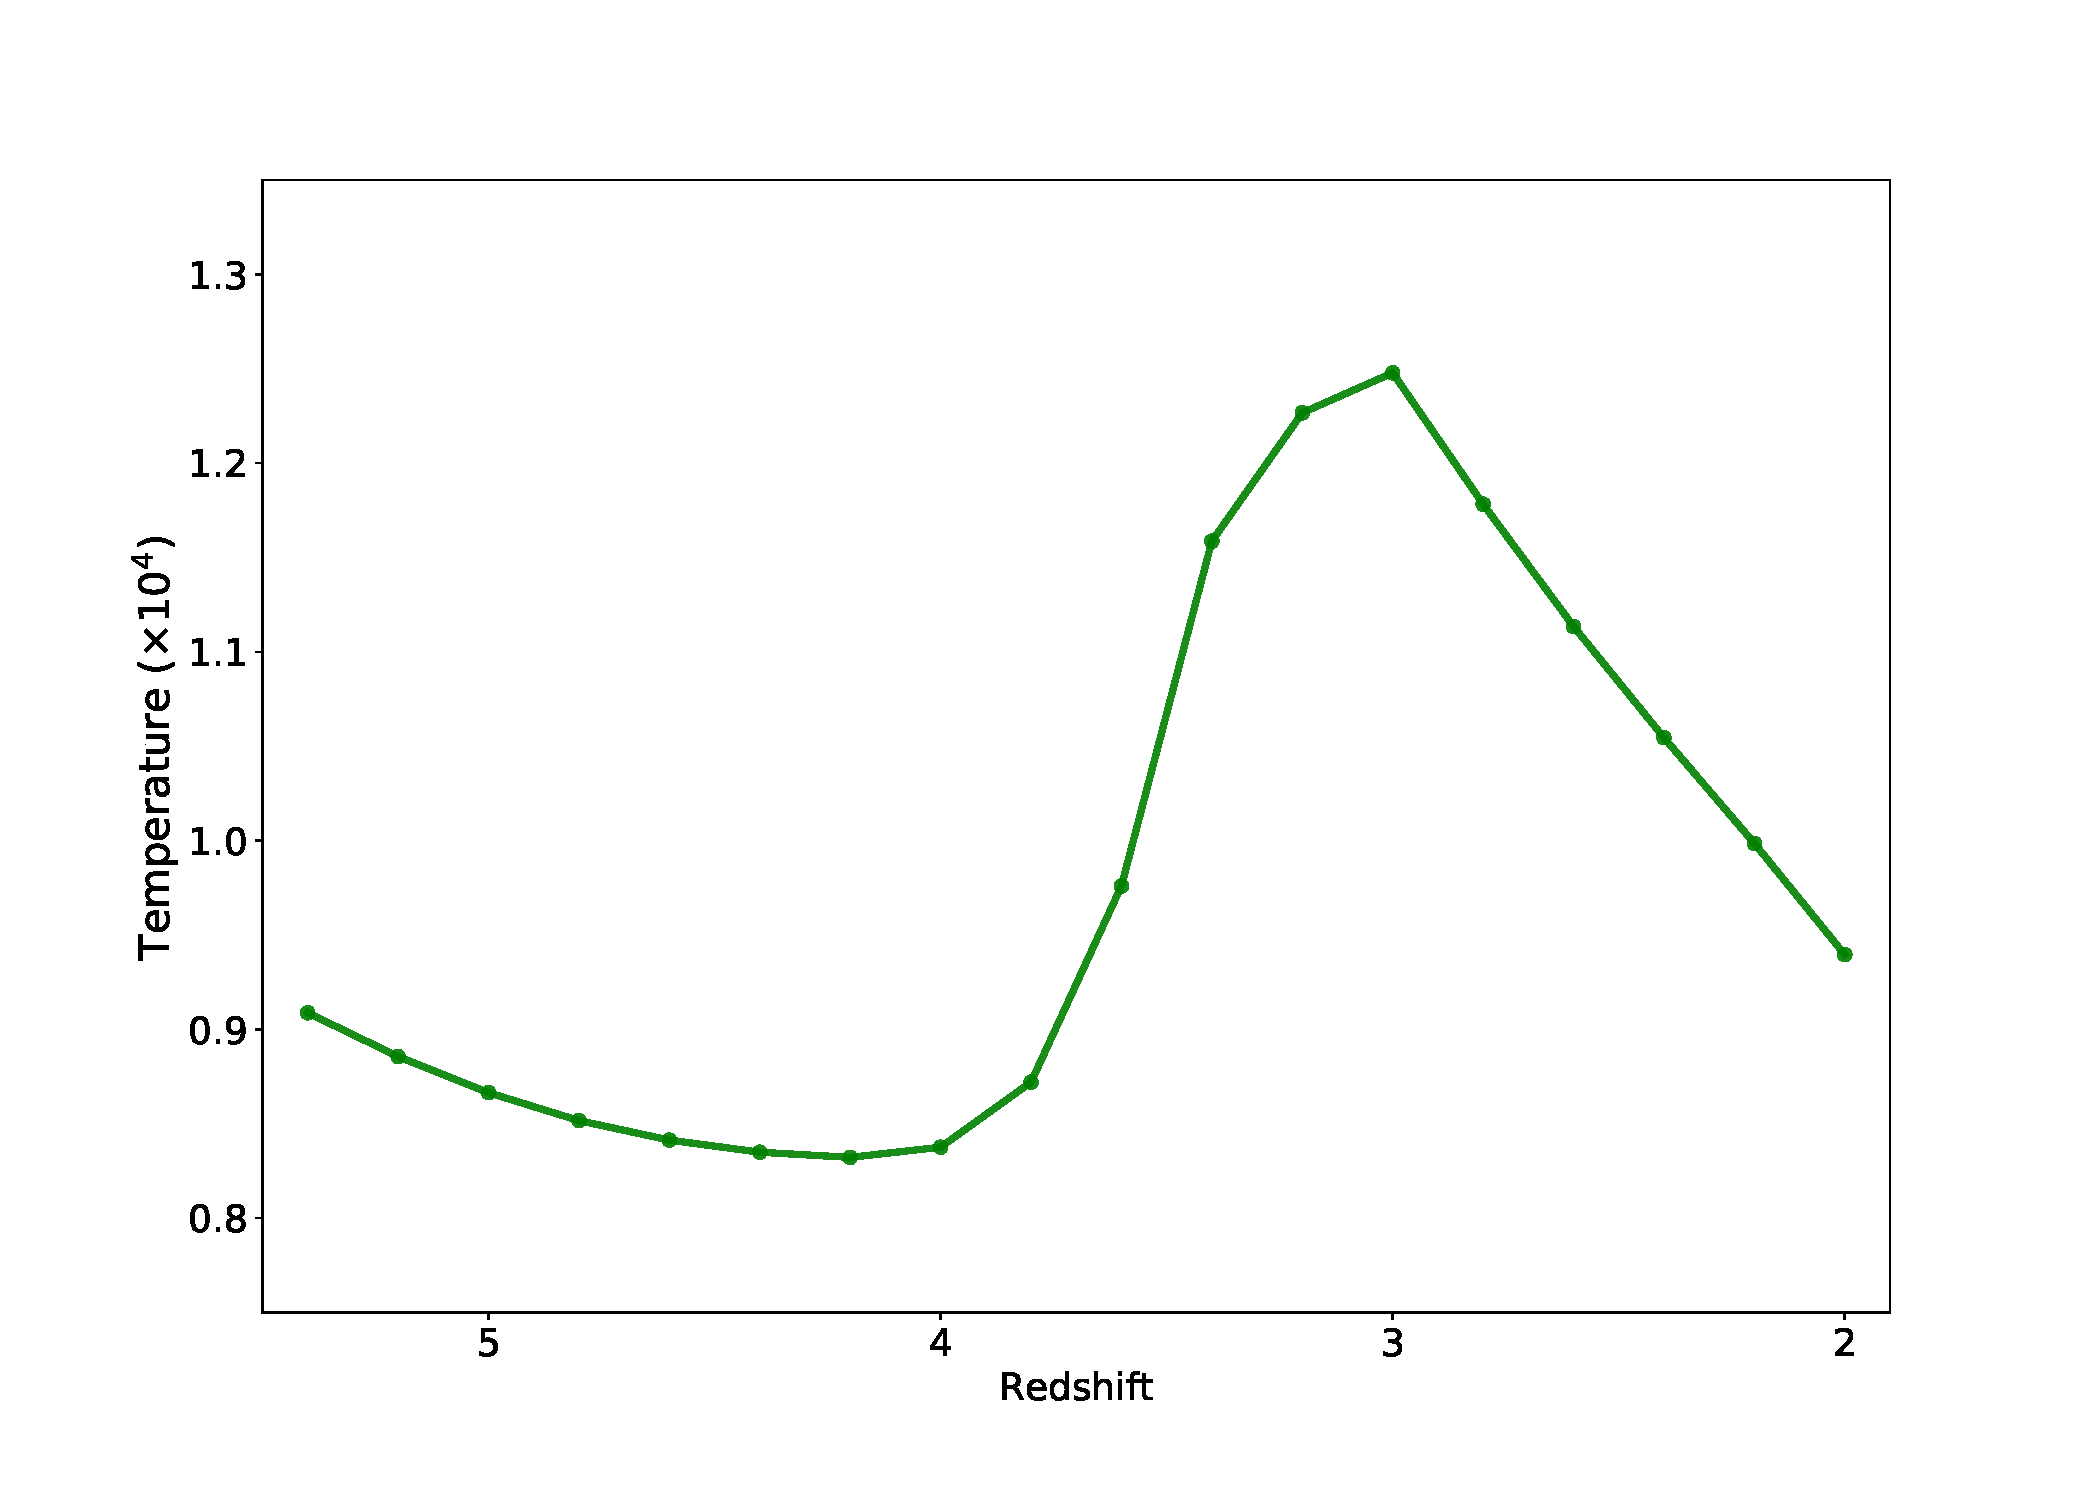
\includegraphics[width=0.45\textwidth]{figures/temps.pdf}
 \caption{Temperature at mean density as a function of redshift. One curve with the largest helium ionization starting redshift, one with the smallest. Then one with the largest $\alpha$ and one with the smallest. Put the mean temperature measurements on the same plot for comparison.}
 \label{fig:heliumtempdens}
\end{figure*}

\begin{figure*}
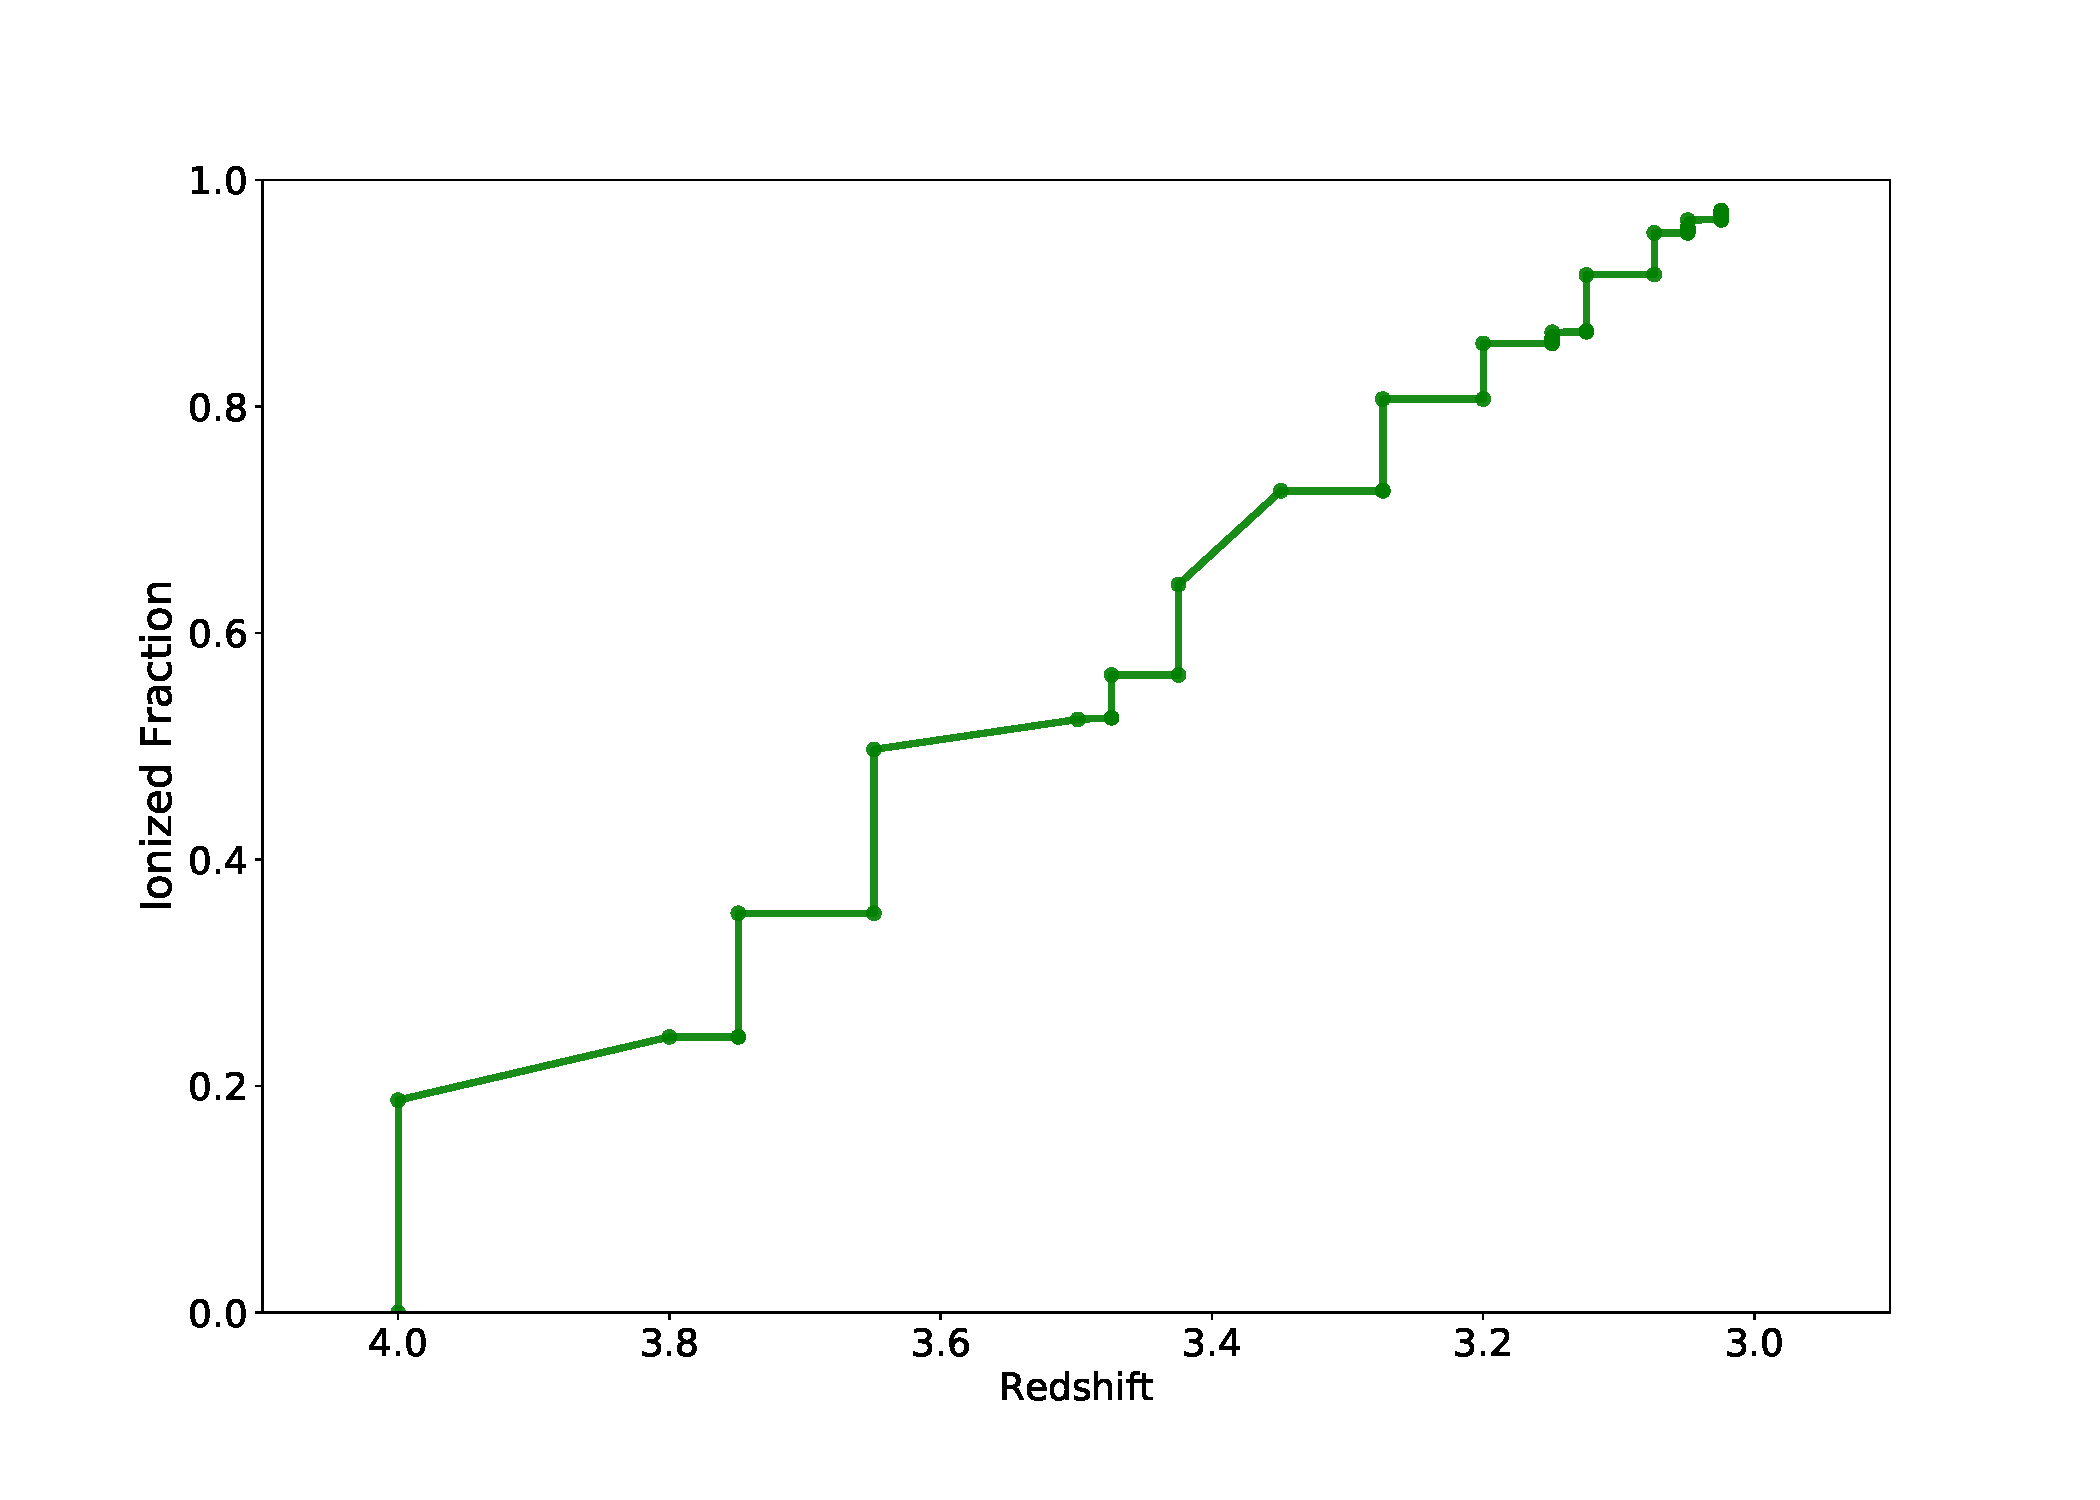
\includegraphics[width=0.45\textwidth]{figures/HeIonFrac.pdf}
 \caption{I don't think we need this one, since it will just be linear in the bigger boxes, but it would be nice to represent the information somewhere anyway for verification. Maybe a lower panel in some other figure?}
 \label{fig:heliumionizationfrac}
\end{figure*}

\begin{figure*}
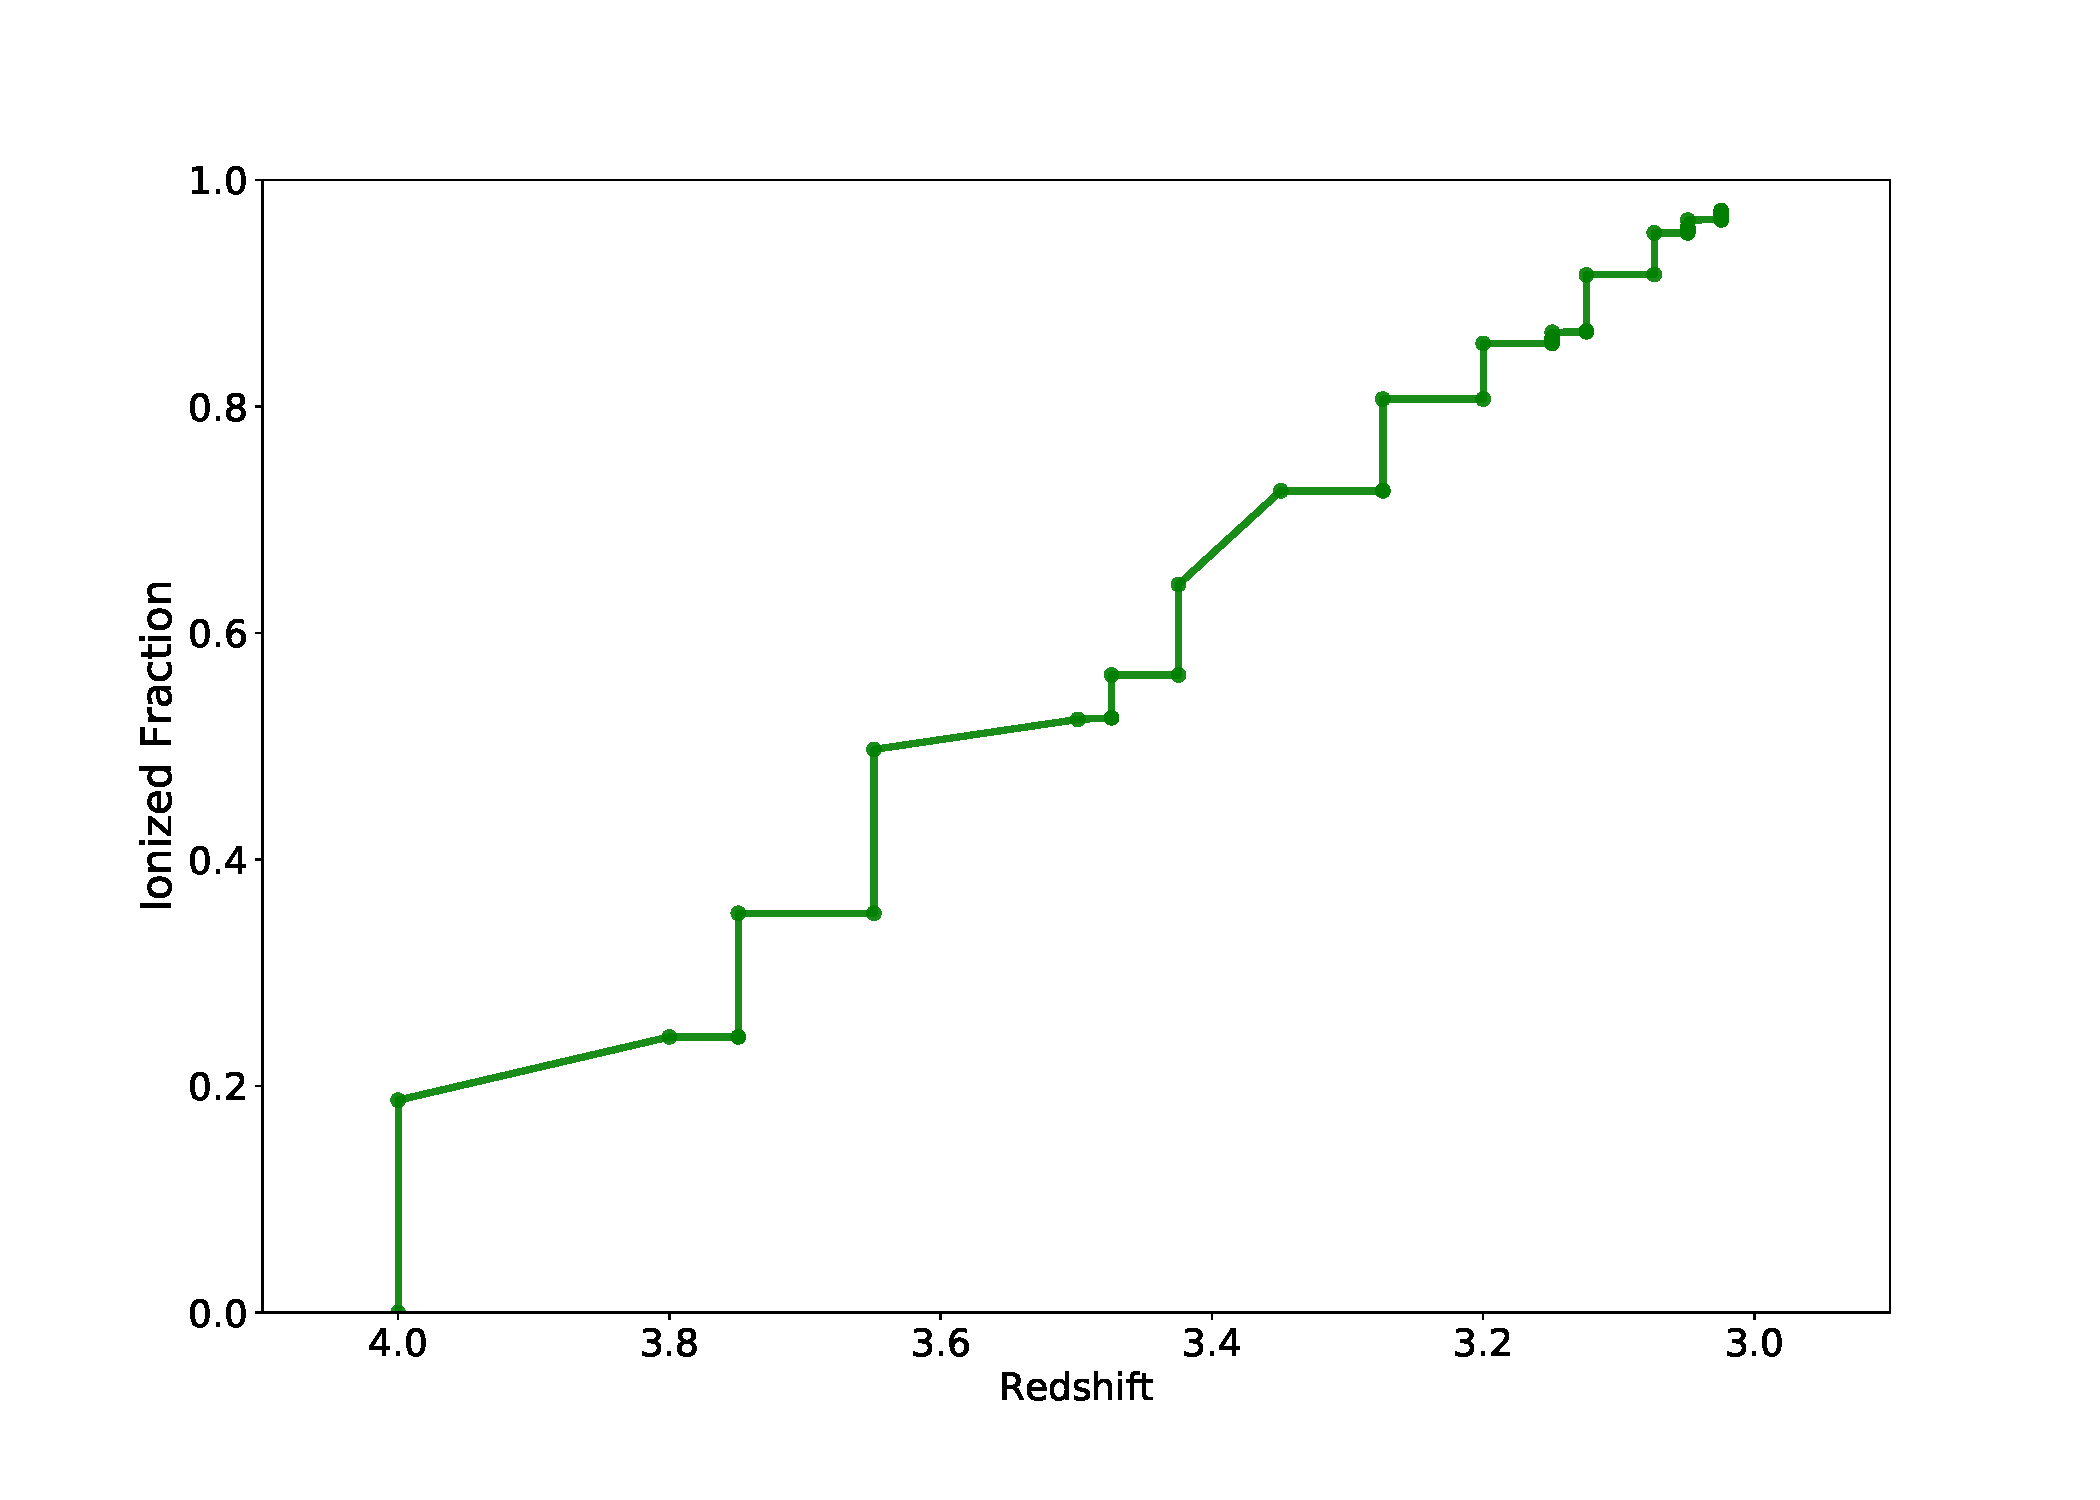
\includegraphics[width=0.45\textwidth]{figures/HeIonFrac.pdf}
 \caption{Show the temperature at mean density for different redshifts of hydrogen reionization. The point is that it has a small ish effect once we get to lower redshifts.}
 \label{fig:hydrogentempdens}
\end{figure*}

\subsection{Star Formation and Stellar Feedback}

\subsection{AGN Feedback}

Plot of the effect of the AGN feedback parameter. Ideally I would compare this to the correction factor from Chabanier et al.

\begin{figure*}
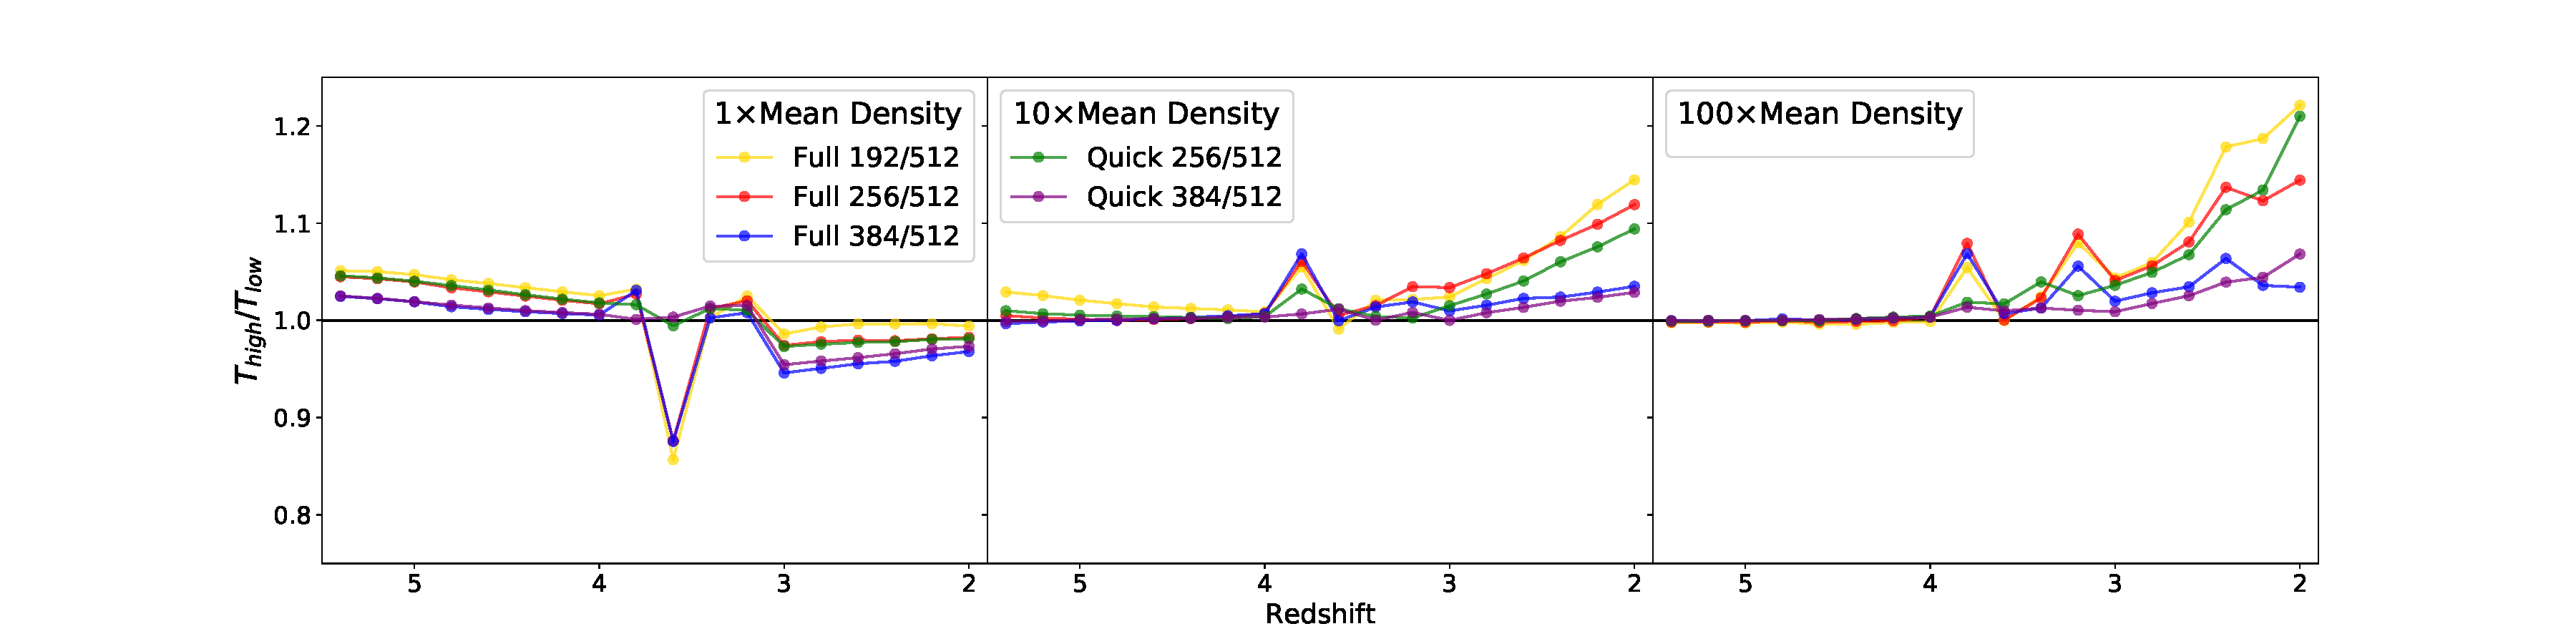
\includegraphics[width=1.\textwidth]{figures/comp-temps_fq.pdf}
 \caption{Temperature variations at different densities for different AGN feedback strengths. Make the point that higher densities are more affected by AGN feedback.}
 \label{fig:AGNtemp}
\end{figure*}

\subsection{Box Size and Particle Load}

Describe the resolution and box size of the simulation. Justify this by citing the relevant 2014 paper and with the figure.

\begin{figure*}
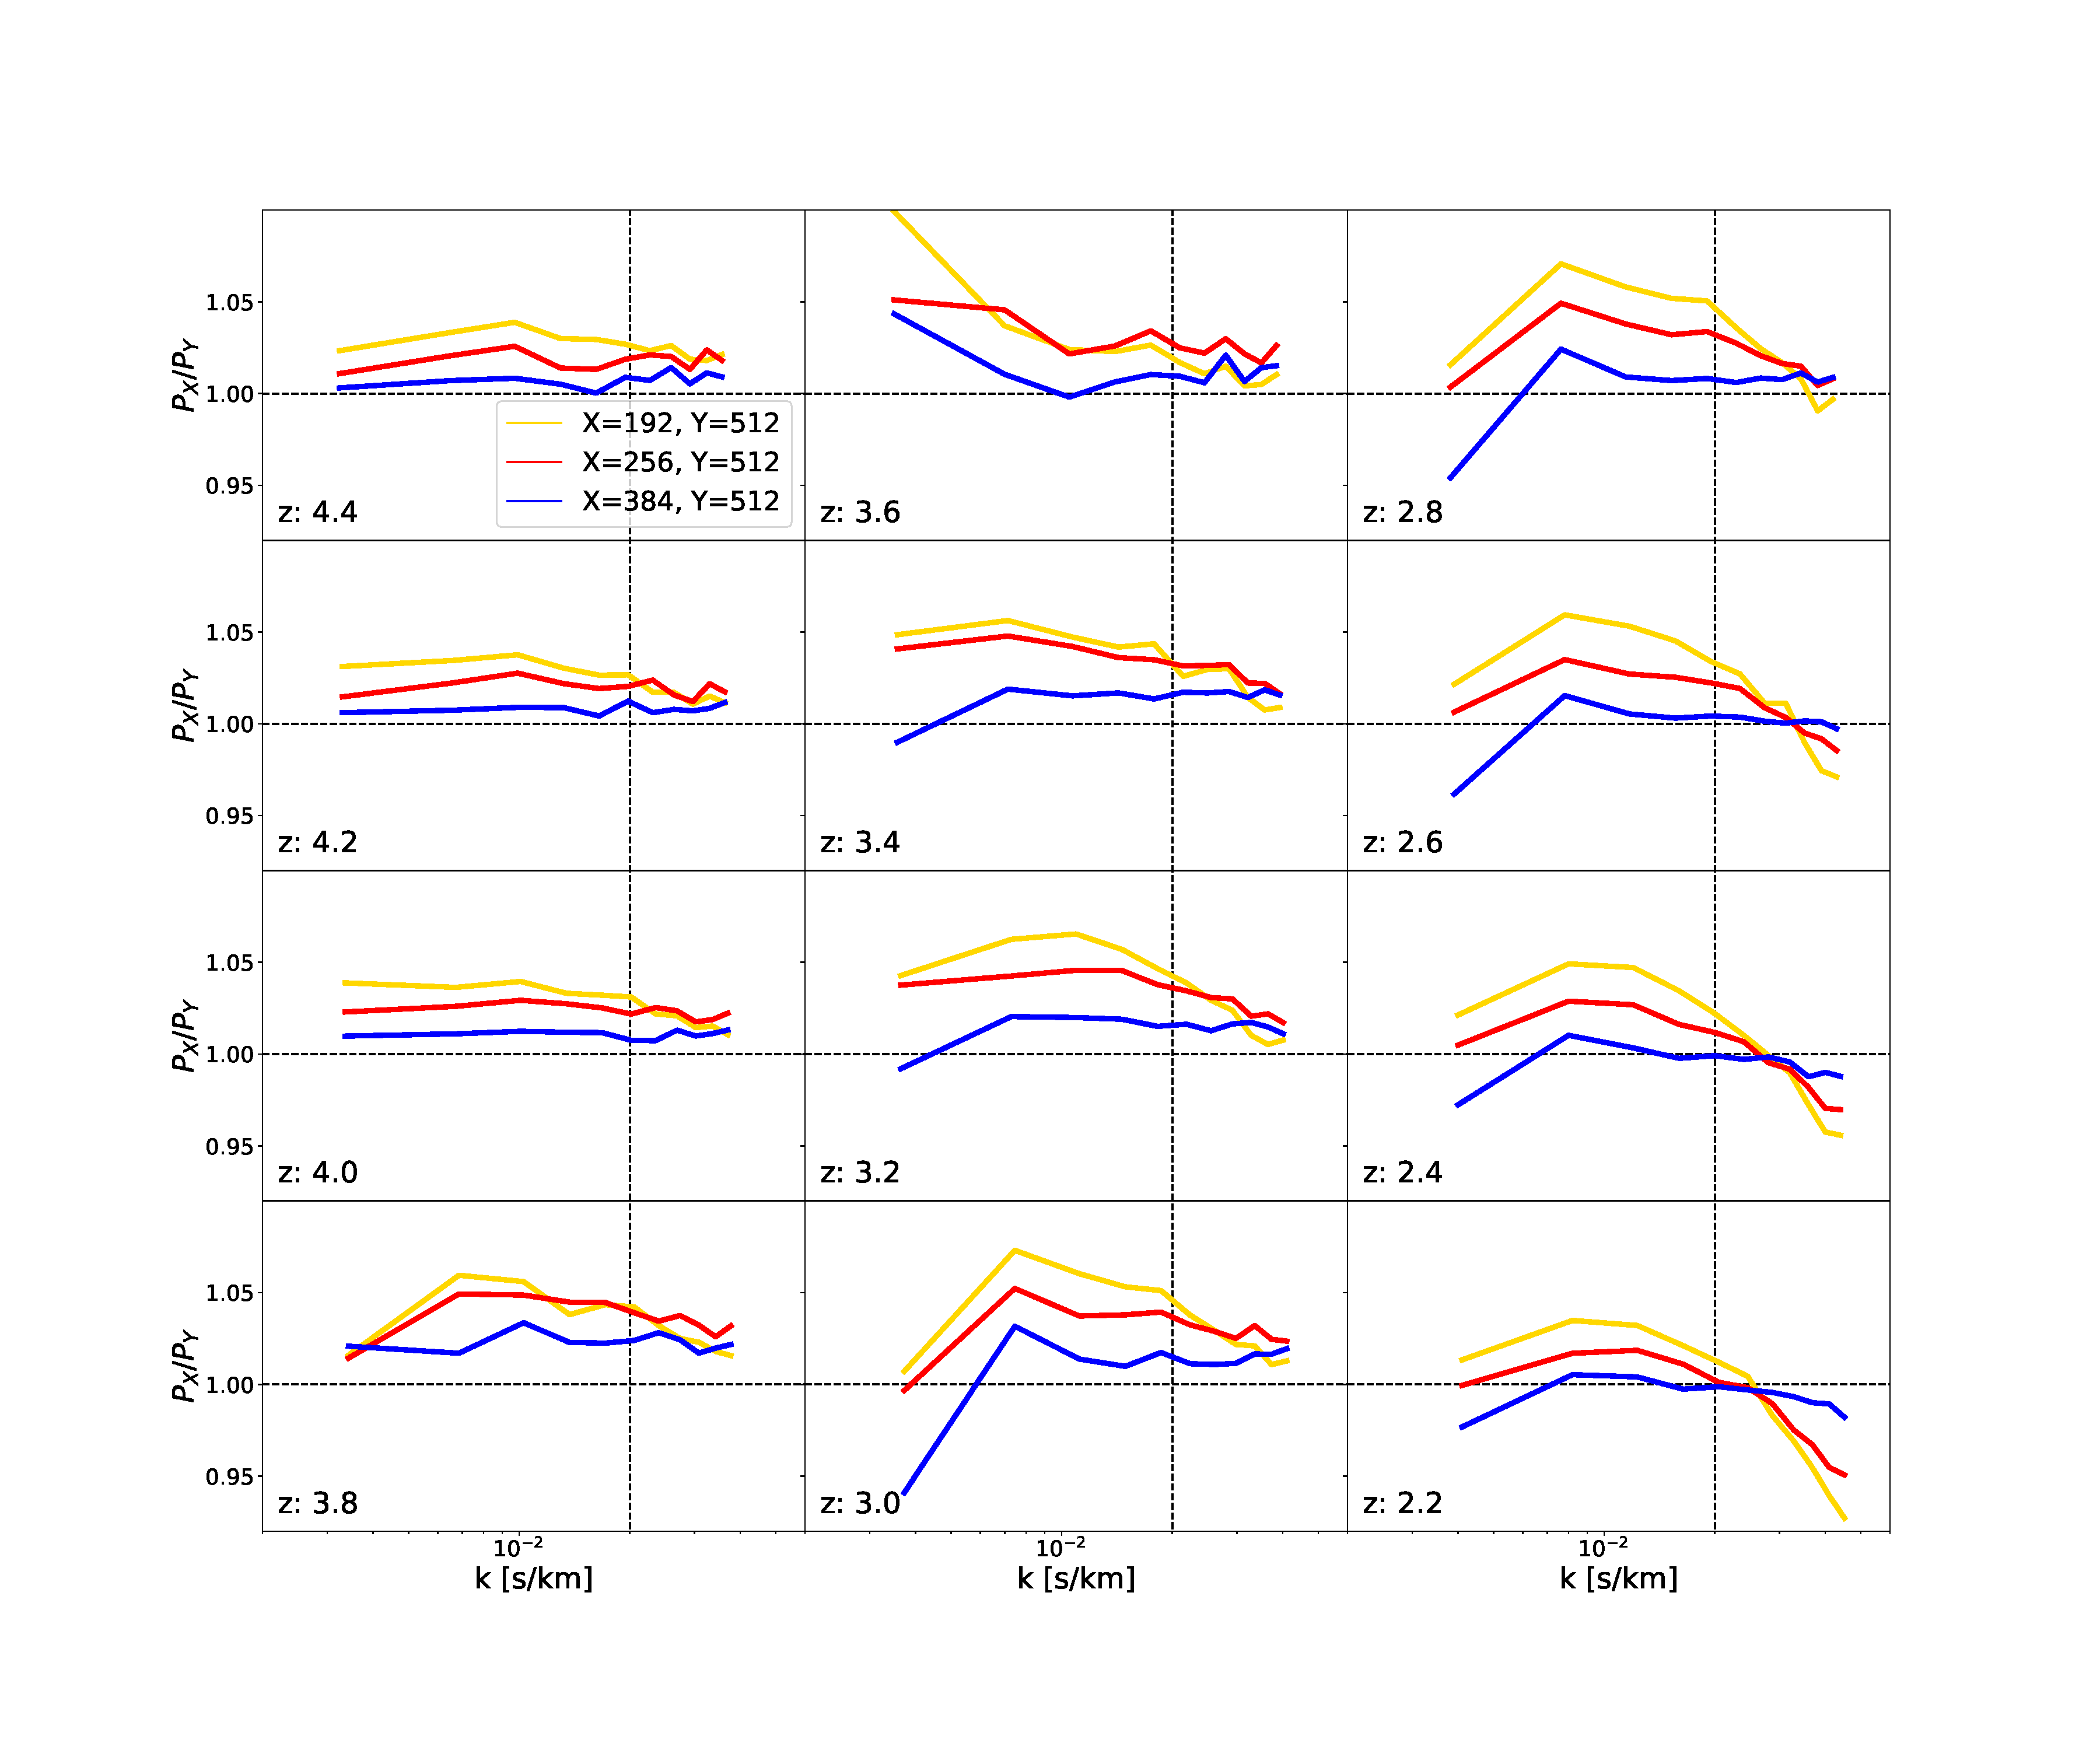
\includegraphics[width=0.45\textwidth]{figures/fps_mfr.pdf}
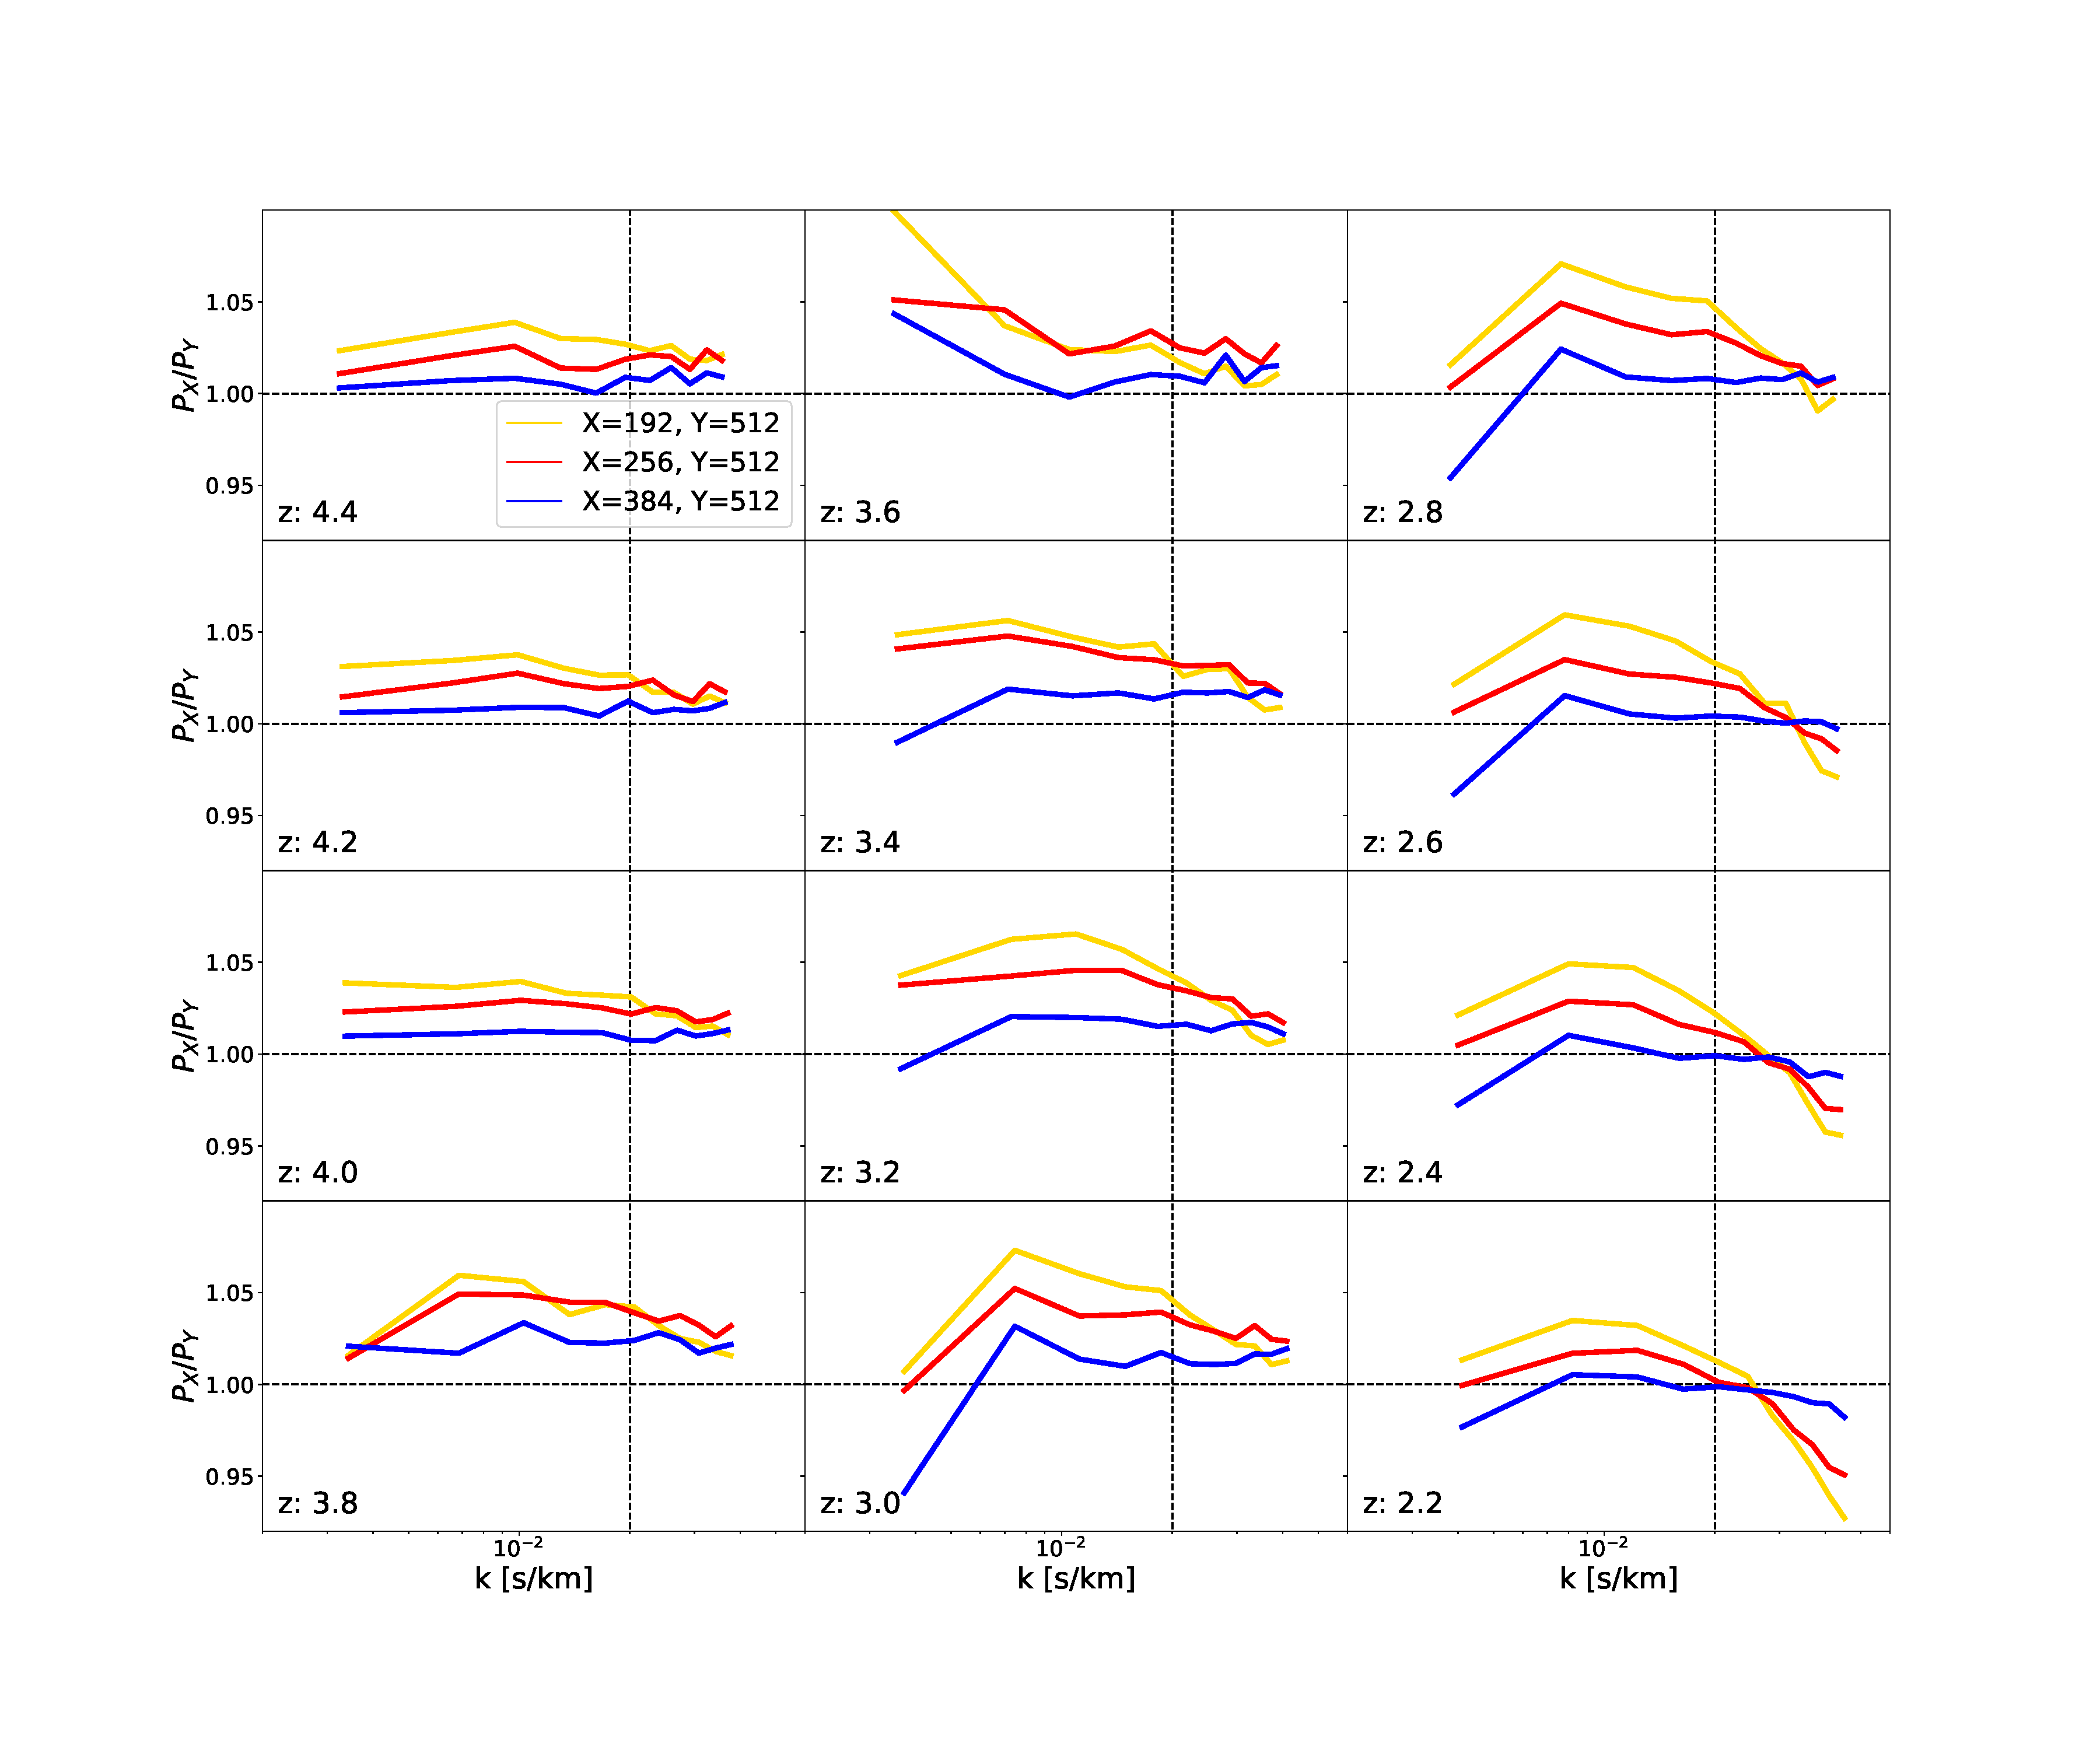
\includegraphics[width=0.45\textwidth]{figures/fps_mfr.pdf}
 \caption{Convergence of the flux power spectrum with resolution and box size. Explain box size and resolution parameters.}
 \label{fig:resolution}
\end{figure*}


\begin{figure*}
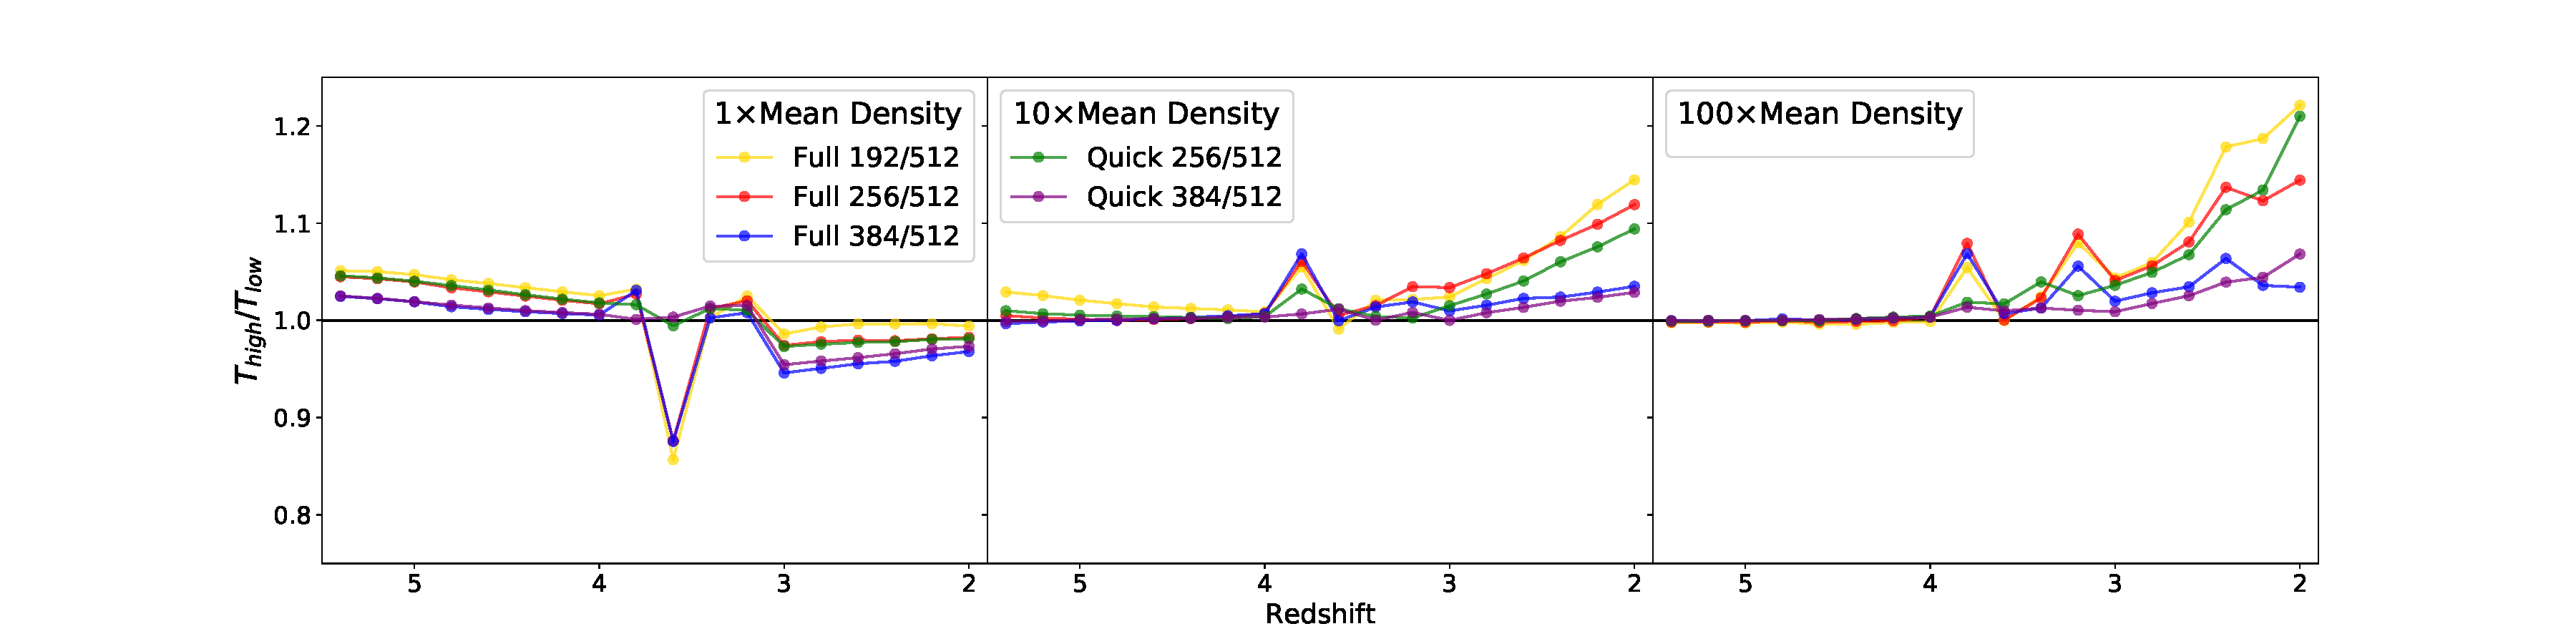
\includegraphics[width=1.\textwidth]{figures/comp-temps_fq.pdf}
 \caption{Temperature variations at different densities for different resolutions. Shows how the convergence changes with redshift.}
 \label{fig:AGNtemp}
\end{figure*}

\section{Simulation Suite Parameters and Experimental Design}

Describe the chosen cosmological parameters. Add a plot as Figure 3 of the multi-fidelity paper. Explain why these parameters are chosen. We use a Latin Hypercube design. Outputs are every $\Delta z=0.2$ from $z=5.4$ to $z=2.0$.

\begin{figure}
    \centering
	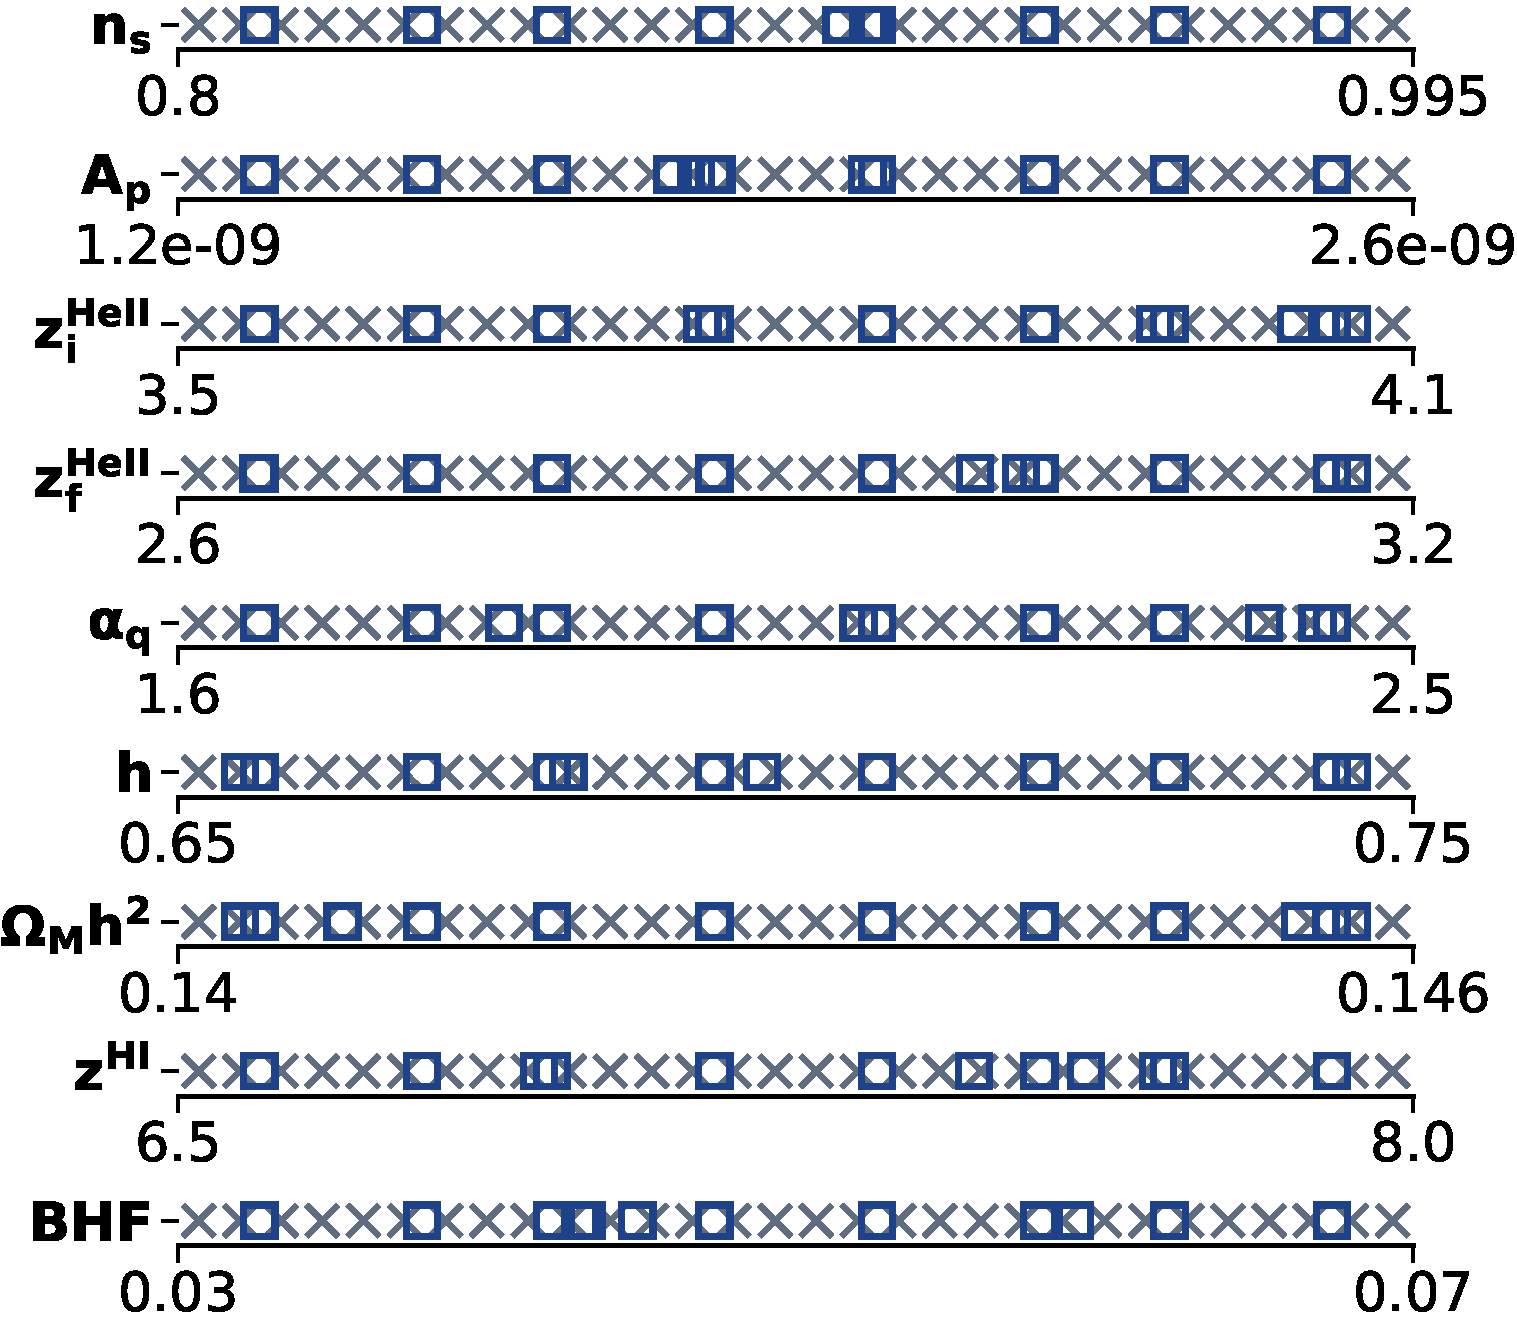
\includegraphics[width=\columnwidth]{figures/120box_42samples.pdf}
    \caption{Simulation parameter limits, and samples used to construct the emulators presented.
    Parameters for the low resolution simulations (crosses) were determined by filling a Latin hypercube.
    From the low resolution set, the optimal high resolution set is determined, and these are shown as red circles.
    Initially, $30$ low resolution samples were generated, then an additional $10$ were added while maintaining the Latin hypercube method, hence the non-uniform spacing for the low resolution samples.}
    \label{fig:samples}
\end{figure}

The emulator construction follows \cite{2019JCAP...02..050B}.

\section{Results}

Plots of the effect of each parameter on the flux power spectrum from the emulator.

\begin{figure}
    \centering
	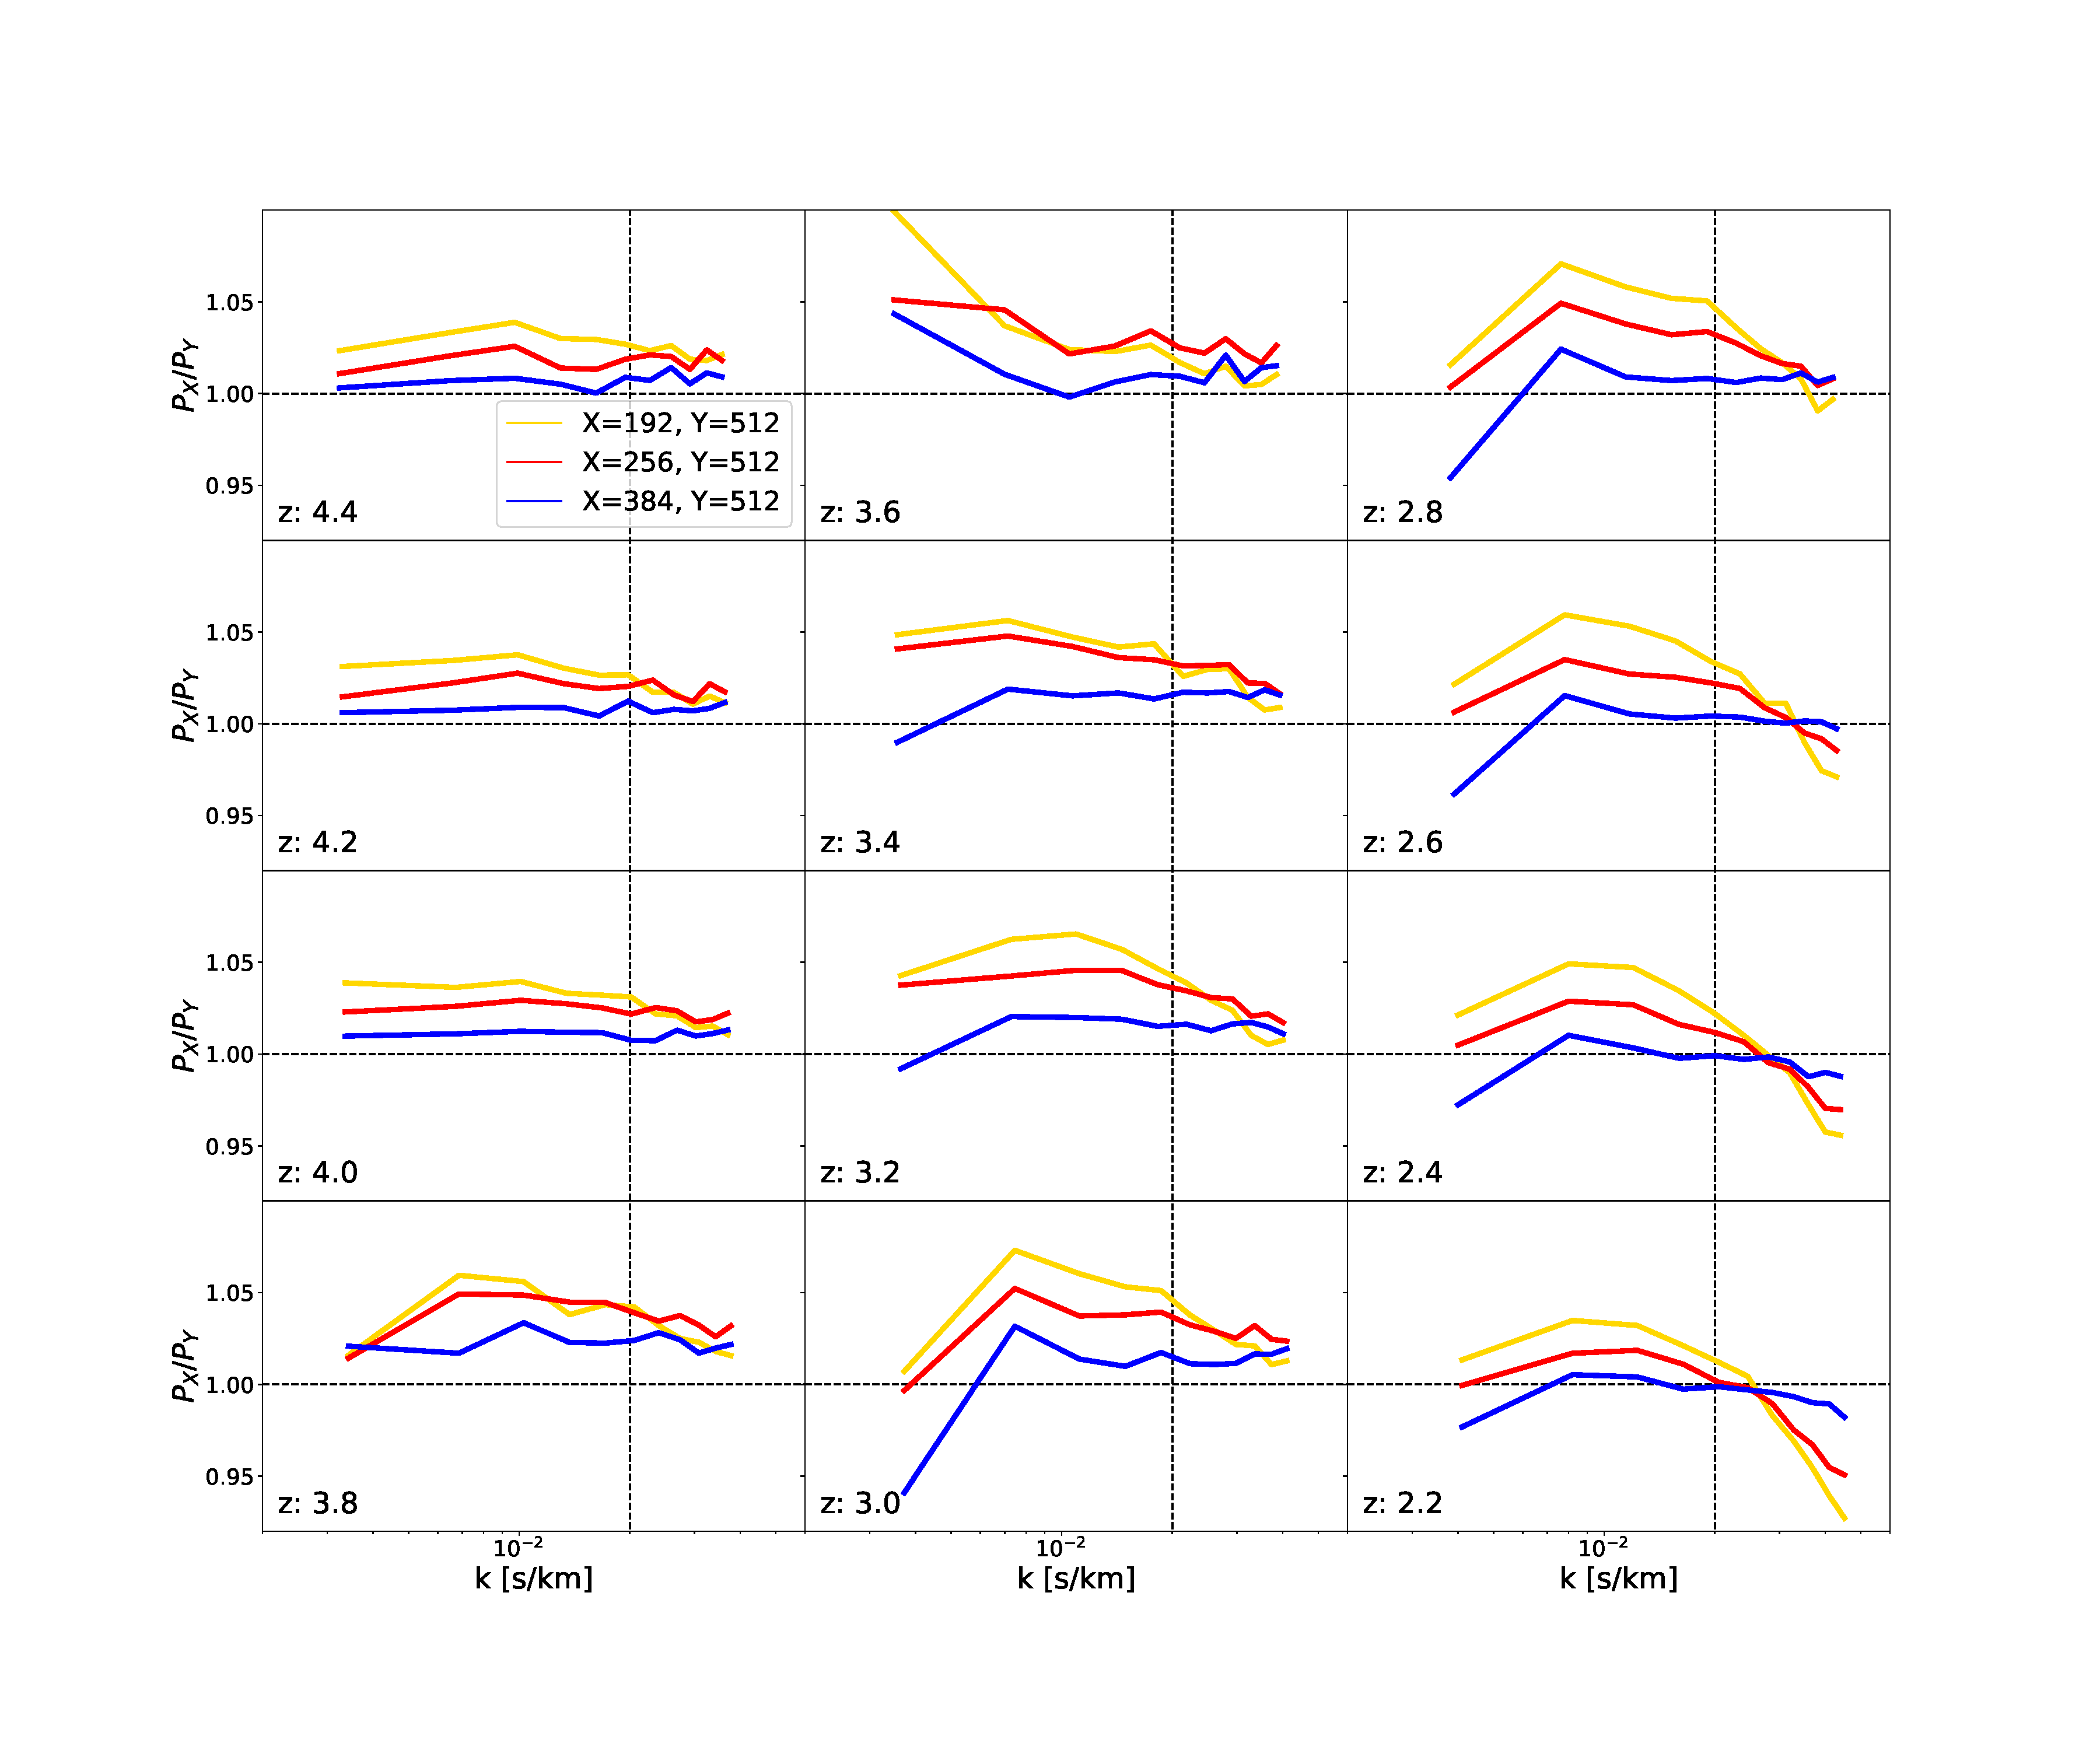
\includegraphics[width=\columnwidth]{figures/fps_mfr.pdf}
    \caption{Effect of changing each simulation parameter on the 1D flux power spectrum at $z=2$ and $z=3$. Plots should look a bit like Figure 9 of \url{https://arxiv.org/pdf/1401.6472.pdf}. Each panel should have 5 lines. Let's have $9$ panels, 1 for each parameter. cosmology parameters ($n_s$, $A_s$, $\Omega_m h^2$, $h$). reionization parameters ($He_i$ and $He_f$, $\alpha_q$, $HI_z$). Finally black hole feedback. }
    \label{fig:fluxpower}
\end{figure}

\section{Conclusion}

Mention multi-fidelity.

\section*{Acknowledgements}
MAF is supported by a National Science Foundation Graduate Research Fellowship under grant No. DGE-1326120.
MFH is supported by a National Aeronautics and Space Administration FINESST under grant No. ASTRO20-0022.
SB is supported by NSF grant AST-1817256.

Computing resources were provided by NSF XSEDE allocation AST21005.
The authors acknowledge the Frontera computing project at the Texas Advanced Computing Center (TACC) for providing HPC and storage resources that have contributed to the research results reported within this paper.
Frontera is made possible by National Science Foundation award OAC-1818253.
URL: \url{http://www.tacc.utexas.edu}

\section*{Data Availability}
Flux power spectra generated from the low resolution, high resolution, and testing sets are available at.
Both HDF5 and plain text (appropriate for multi-fidelity emulation) formats are available.
Single- and multi-fidelity emulator predictions for the $10$ testing simulations are also available from the same repository.
The spectra underlying the flux power are available upon request.

\bibliographystyle{JHEP}
\bibliography{refs}

\appendix

\label{lastpage}
\end{document}
